\documentclass[12pt]{standalone}
\usepackage{tikz}
\usepackage{amsmath}
\usetikzlibrary{arrows.meta, calc, decorations.pathreplacing}

% ─────────────────────────────────────────────────────────────────
%  Color definitions
% ─────────────────────────────────────────────────────────────────
\definecolor{refblue}    {RGB}{24,  95, 165}   % reference frame blue
\definecolor{refbluefill}{RGB}{181,212,244}
\definecolor{currteal}   {RGB}{ 15,110, 86}    % current frame teal
\definecolor{currtealfill}{RGB}{159,225,203}
\definecolor{mappingred} {RGB}{163, 45,  45}
\definecolor{circgray}   {RGB}{ 95, 94, 90}
\definecolor{axiscolor}  {RGB}{ 95, 94, 90}

\begin{document}
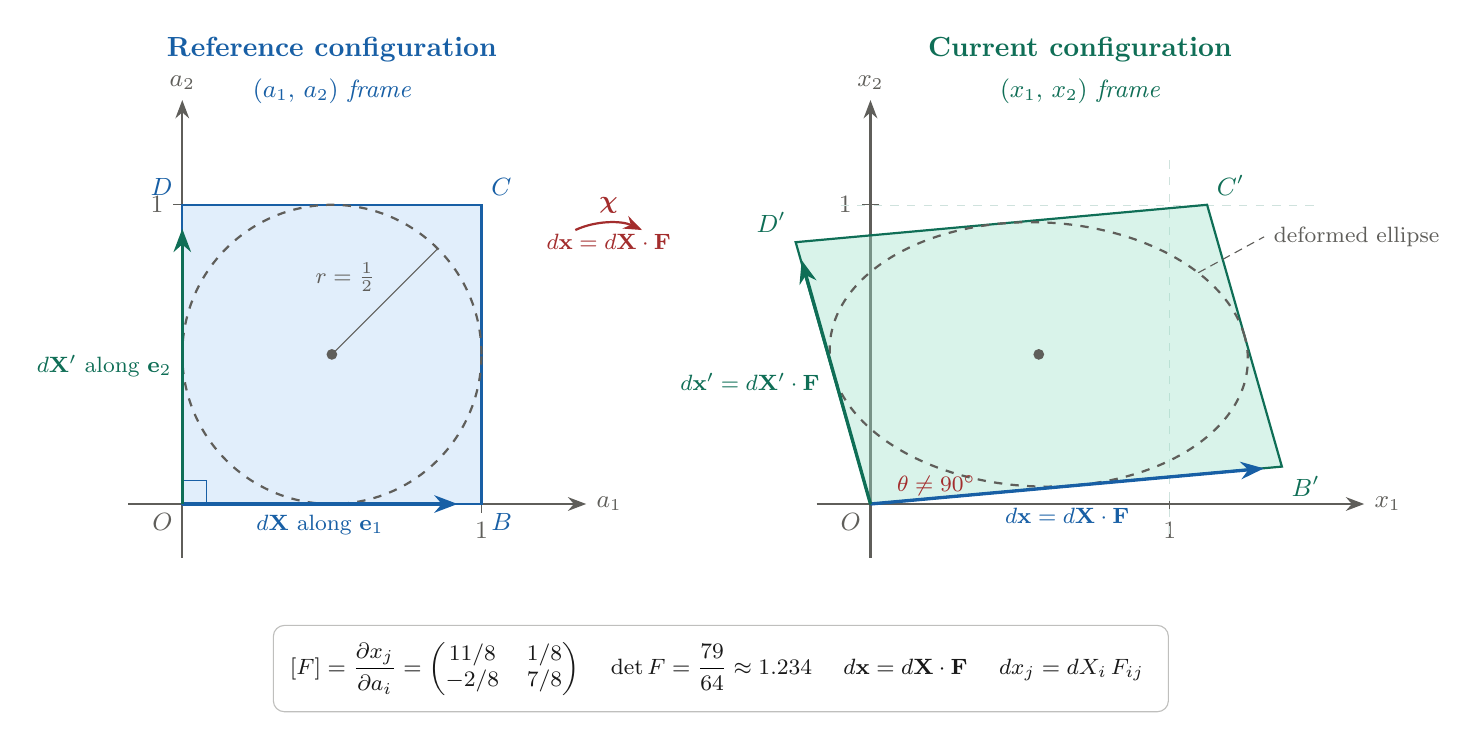
\begin{tikzpicture}[
    scale      = 3.8,           % 1 unit = 3.8 cm  (generous for A4 / beamer)
    >=Stealth,
    every node/.style = {font=\small},
    axis/.style       = {->, thick, axiscolor},
    fiber/.style      = {->, very thick},
    leader/.style     = {densely dashed, thin, circgray},
    mapArrow/.style   = {->, thick, mappingred,
                         bend left=30, shorten >=4pt, shorten <=4pt}
]

% ═══════════════════════════════════════════════════════════════
%  REFERENCE CONFIGURATION  —  origin OR = (0,0)
% ═══════════════════════════════════════════════════════════════

% --- coordinate axes ---
\draw[axis] (-0.18, 0) -- (1.35, 0) node[right] {$a_1$};
\draw[axis] ( 0, -0.18) -- (0, 1.35) node[above] {$a_2$};
\node[below left, axiscolor] at (0,0) {$O$};

% tick marks
\draw[thin,axiscolor] (1, 0.03) -- (1,-0.03) node[below] {$1$};
\draw[thin,axiscolor] (0.03,1) -- (-0.03,1) node[left]  {$1$};

% --- light grid ---
\draw[very thin, refblue!25] (1,0) -- (1,1);
\draw[very thin, refblue!25] (0,1) -- (1,1);

% --- unit square (filled) ---
\fill[refbluefill, fill opacity=0.4]  (0,0) -- (1,0) -- (1,1) -- (0,1) -- cycle;
\draw[refblue, thick]                 (0,0) -- (1,0) -- (1,1) -- (0,1) -- cycle;

% right-angle marker at A
\draw[refblue, thin] (0.08,0) -- (0.08,0.08) -- (0,0.08);

% corner labels
%\node[below left,  refblue] at (0,0) {$A$};
\node[below right, refblue] at (1,0) {$B$};
\node[above right, refblue] at (1,1) {$C$};
\node[above left,  refblue] at (0,1) {$D$};

% --- inscribed circle (r=1/2, centre (1/2,1/2)) ---
\draw[circgray, thick, dashed] (0.5, 0.5) circle [radius=0.5];
\fill[circgray] (0.5,0.5) circle [radius=0.018];
\draw[thin, circgray] (0.5,0.5) -- +(45:0.5)
    node[midway, above left, circgray, font=\footnotesize] {$r=\tfrac{1}{2}$};

% --- fiber vectors along edges ---
% e1 direction (A→B)
\draw[fiber, refblue]
    (0,0) -- (0.92,0)
    node[midway, below, refblue, font=\footnotesize] {$d\mathbf{X}$ along $\mathbf{e}_1$};
% e2 direction (A→D)
\draw[fiber, currteal]
    (0,0) -- (0, 0.92)
    node[midway, left, currteal, font=\footnotesize] {$d\mathbf{X}'$ along $\mathbf{e}_2$};

% panel title
\node[refblue, font=\normalsize\bfseries] at (0.5, 1.52)
    {Reference configuration};
\node[refblue, font=\small\itshape] at (0.5, 1.38)
    {$(a_1,\,a_2)$ frame};

% ═══════════════════════════════════════════════════════════════
%  MAPPING ARROW  (between the two panels)
% ═══════════════════════════════════════════════════════════════
% Panels are separated by ~0.55 units gap (ref right edge at x=1,
% current left edge starts at x=1.55 in the shifted frame below).
% The arrow goes from approx (1.08, 0.85) to (1.47, 0.85).

\draw[mapArrow, font=\normalsize]
    (1.28, 0.90) to [bend left=25] node[above, mappingred]
        {$\boldsymbol{\chi}$} node[below, mappingred, font=\footnotesize]
        {$d\mathbf{x} = d\mathbf{X}\cdot\mathbf{F}$}
    (1.57, 0.90);

% ═══════════════════════════════════════════════════════════════
%  CURRENT CONFIGURATION  —  origin OC shifted to (1.55, 0)
% ═══════════════════════════════════════════════════════════════
%
%  Deformation mapping:  x_j = X_i F_{ij}
%    F = [ 11/8   1/8 ]    (row i, column j)
%        [ -2/8   7/8 ]
%
%  Mapped corners  (X_i F_{ij}):
%    A(0,0) -> (0,       0      )
%    B(1,0) -> (11/8,    1/8   )
%    C(1,1) -> (11/8-2/8, 1/8+7/8) = (9/8, 8/8) = (9/8, 1)
%    D(0,1) -> (-2/8,    7/8   )
%
%  All coordinates below are RELATIVE to the current origin OC.
%  In the picture we add the shift (1.55, 0) via the scope.

\begin{scope}[xshift=2.3cm] 
% cleaner: just use xshift in units of the current scale


% --- coordinate axes ---
\draw[axis] (-0.18, 0) -- (1.65, 0) node[right] {$x_1$};
\draw[axis] ( 0, -0.18) -- (0, 1.35) node[above] {$x_2$};
\node[below left, axiscolor] at (0,0) {$O$};

% tick marks (unit length guides)
\draw[thin,axiscolor] (1, 0.03) -- (1,-0.03) node[below] {$1$};
\draw[thin,axiscolor] (0.03,1) -- (-0.03,1) node[left]  {$1$};

% light dashed reference grid
\draw[very thin, currteal!20, dashed] (1,-0.1) -- (1,1.15);
\draw[very thin, currteal!20, dashed] (-0.1,1) -- (1.5,1);

% --- deformed parallelogram (filled) ---
%  A'=(0,0)  B'=(11/8, 1/8)  C'=(9/8, 1)  D'=(-2/8, 7/8)
\fill[currtealfill, fill opacity=0.4]
    (0,0) -- (11/8, 1/8) -- (9/8, 1) -- (-2/8, 7/8) -- cycle;
\draw[currteal, thick]
    (0,0) -- (11/8, 1/8) -- (9/8, 1) -- (-2/8, 7/8) -- cycle;

% corner labels
%\node[below left,  currteal] at (0,    0   ) {$A'$};
\node[below right, currteal] at (11/8, 1/8 ) {$B'$};
\node[above right, currteal] at (9/8,  1   ) {$C'$};
\node[above left,  currteal] at (-2/8, 7/8 ) {$D'$};

% --- deformed ellipse ---
% Parametric:
%   x1(t) = 9/16 + 1/2*(11/8 cos t - 2/8 sin t)
%   x2(t) = 1/2  + 1/2*(1/8  cos t + 7/8 sin t)
% TikZ parametric plot (t in degrees)
\draw[circgray, thick, dashed,
      samples=120, smooth, variable=\t, domain=0:360]
    plot ({9/16 + 0.5*(11/8*cos(\t) - 2/8*sin(\t))},
          {1/2  + 0.5*( 1/8*cos(\t) + 7/8*sin(\t))});

% ellipse centre
\fill[circgray]
    ({9/16}, {1/2}) circle [radius=0.018];

% leader to ellipse label
\draw[leader]
    ({9/16 + 0.5*(11/8*cos(30) - 2/8*sin(30))},
     {1/2  + 0.5*( 1/8*cos(30) + 7/8*sin(30))})
    -- +(0.22, 0.12)
    node[right, circgray, font=\footnotesize]
        {deformed ellipse};

% leader to circle label (in reference, carried over as annotation)
% (annotated directly on reference panel already)

% --- no-longer-right-angle annotation ---
\node[mappingred, font=\footnotesize] at (0.22, 0.06) {$\theta \neq 90^{\circ}$};

% --- fiber vectors (images of basis vectors) ---
% Image of e1:  row 1 of F = (11/8, 1/8)
\draw[fiber, refblue]
    (0,0) -- ({11/8 - 0.06}, {1/8 - 0.006})
    node[midway, below=4pt, refblue, font=\footnotesize]
        {$d\mathbf{x}=d\mathbf{X}\cdot\mathbf{F}$};
% Image of e2:  row 2 of F = (-2/8, 7/8)
\draw[fiber, currteal]
    (0,0) -- ({-2/8 + 0.02}, {7/8 - 0.06})
    node[midway, left=2pt, currteal, font=\footnotesize]
        {$d\mathbf{x}'=d\mathbf{X}'\cdot\mathbf{F}$};

% panel title
\node[currteal, font=\normalsize\bfseries] at (0.7, 1.52)
    {Current configuration};
\node[currteal, font=\small\itshape] at (0.7, 1.38)
    {$(x_1,\,x_2)$ frame};

\end{scope}

% ═══════════════════════════════════════════════════════════════
%  ANNOTATION BOX  (below, centred on the whole figure)
% ═══════════════════════════════════════════════════════════════
\node[draw=axiscolor!40, fill=white, fill opacity=0.9,
      rounded corners=4pt, inner sep=6pt,
      font=\footnotesize, align=center]
at (1.8, -0.55)   % in cm, centred between the two panels
{
$[F] = \dfrac{\partial x_j}{\partial a_i} =
\begin{pmatrix} 11/8 & 1/8 \\ -2/8 & 7/8 \end{pmatrix}$
\quad
$\det F = \dfrac{79}{64} \approx 1.234$
\quad
$d\mathbf{x} = d\mathbf{X}\cdot\mathbf{F}$
\quad
$dx_j = dX_i\,F_{ij}$
};

\end{tikzpicture}
\end{document}
